\documentclass[a4paper]{jpconf}
\usepackage{graphicx}
\usepackage{color}
\usepackage{array}
\newcommand{\cred}[1]{{\color{red}#1}}

\begin{document}
\title{Vibrational characteristics of a superconducting magnetic bearing employed for a prototype polarization modulator}

\author{Yuki Sakurai$^{1}$, Tomotake Matsumura$^{1}$, Hajime Sugai$^{1}$, Nobuhiko Katayama$^{1}$, Hiroyuki Ohsaki$^{2}$, Yutaka Terao$^{2}$, Yusuke Terachi$^{2}$, Hirokazu Kataza$^{3}$, Shin Utsunomiya$^{1}$, Ryo Yamamoto$^{3}$}
\vspace{2mm}
\address{
$^{1}$Kavli Institute for the Physics and Mathematics of the Universe (WPI),The University of Tokyo Institutes for Advanced Study, The University of Tokyo, 5-1-5 Kashiwanoha, Kashiwa, Chiba 277-8583, Japan \\
$^{2}$Graduate School of Frontier Sciences, The University of Tokyo, 5-1-5 Kashiwanoha, Kashiwa, Chiba 277-8561, Japan \\
$^{3}$Japan Aerospace Exploration Agency, Institute of Space and Astronautical Science (ISAS), 3-1-1 Yoshinodai, Chuo-ku, Sagamihara, Kanagawa 252-5210, Japan
}

\ead{yuki.sakurai@ipmu.jp, tomotake.matsumura@ipmu.jp}

\begin{abstract}
We present the vibrational characteristics of a levitating rotor in a superconducting magnetic bearing (SMB) system operating at below 10~K.
We develop a polarization modulator that requires a continuously rotating optical element, called half-wave plate (HWP), for a cosmic microwave background polarization experiment.
The HWP has to operate at the temperature below 10~K, and thus an SMB provides a smooth rotation of the HWP at the cryogenic temperature of about 10~K with minimal heat dissipation.
In order to understand the potential interference to the cosmological observations due to the vibration of the HWP,
it is essential to characterize the vibrational properties of the levitating rotor of the SMB.
We constructed a prototype model that consists of an SMB with an array of high temperature superconductors, YBCO, and a permanent magnet ring, NdFeB.
The rotor position is monitored by a laser displacement gauge, and a cryogenic Hall sensor via the magnetic field.
In this presentation, we present the measurement results of the vibration characteristics using our prototype SMB system.
%We discuss the measurement of the spring constant using our prototype system.
%and the magnetic field inhomogeneity of the SMB and sub-components including a rotation frequency monitoring system, a holder mechanism, and drive system.
We characterize the vibrational properties as the spring constant and the damping, and discuss the projected performance of this technology toward the use in future space missions.
\end{abstract}

\section*{Introduction}

A cosmic microwave background (CMB) is electromagnetic microwave radiation from the big bang.
It is still observable isotropically from the whole sky today.
One of most important research topics in the current cosmology and high-energy physics is to study the cosmic inflation theory, which predicts a rapid expansion of the universe after $\sim 10^{-38}$ seconds from the beginning of the universe~\cite{inflation_sato,inflation_guth}.
The inflation solves several mysteries of the standard cosmology and it can provide a foothold for new physics in high energy physics.
The theory predicts that the inflation left the divergence free pattern in the CMB polarization,  called "B-mode".
Therefore, the experimental discovery of the cosmic inflation is possible by observing the CMB B-mode polarization.
A world-wide keen discovery race is spreading among many CMB polarization experiments.
Correspondingly, the instrumental development has progressed remarkably.

One of the critical instruments for a precise measurement of the CMB polarization is a "polarization modulator".
It consists of an optical element, a half-wave plate (HWP), and a rotational mechanism.
The continuously rotating HWP modulates the CMB polarization signal synchronously at the four times of the rotational frequency of the HWP, a few Hz.
%Since the intrinsic instrumental noise is not modulated, systematic uncertainties are significantly reduced.
The continuously rotating HWP have to be maintained at cryogenic temperature ($\sim$ 10~K) in order to reduce the detector noise originating from the excess thermal emission of the HWP itself to the detector.
It is therefore necessary to use a rotational mechanism which allows to rotate with minimal heat dissipation at cryogenic temperature.

An superconducting magnetic bearing (SMB) is a contactless bearing~\cite{smb}.
it employs an array of high temperature superconductor tiles as a stator and a permanent magnet as a rotor.
The rotor levitates above a stator and spins without contact.
There is no friction due to the physical contact, and thus this technology is well matched for use in the polarization modulator, which is required to operate at the cryogenic temperature with minimal heat dissipation.
%In general mechanical bearings produces too much heat due to friction from a physical contact.
%Thus, a superconducting magnetic bearing (SMB) is a good candidate for the rotational mechanism~\cite{smb}.
%The SMB is a rotational bearing utilizing magnetic levitation by the type II superconductor and the magnetic field from a permanent magnet, and thus there is no physical contact between a rotor and a stator.
This unique application is first investigated for use in a balloon-borne CMB polarization experiment, called EBEX~\cite{ebex}.
The successful implementation accelerates the interest for further development toward the next generation experiment from a ground telescope to a satellite mission~\cite{litebird}.

While the heat dissipation is expected to be smaller than that from a conventional mechanical bearing, the stiffness of the rotor over the stator is expected to be less rigid as compare to the mechanical bearing.
Therefore, the levitation based bearing has an inherent trade-off between the heat dissipation and the stiffness.
In this paper, we discuss the design trade-off for use of this SMB technology for a future CMB polarization experiment.
We present our prototype SMB system, rotor diameter of 384~mm, and the measurements of the spring constant and the damping coefficient to characterize the mechanical properties.
In order to characterize the mechanical properties, we use a laser displacement gauge, which we can use in a lab but cannot use during observations.
As an alternative solution, we also introduce a Hall sensor to monitor the mechanical properties simultaneously.
We discuss the consistency between the two independent measurements and propose the concise passive technic to monitor the vibrational motion of the rotor magnet at the cryogenic temperature.
Finally we projects the results toward the design of the SMB system for the polarization modulator.
%\cred{tomo: continue editing from here}It is possible to achieve minimal heat dissipation at cryogenic temperature with the SMB.
%The SMB is developed mainly for industries such as flywheel energy storage,
%although the polarization modulator is one of unique applications and it plays critical role in the CMB polarization experiments.
%A balloon experiment called EBEX has succeeded the CMB polarization observation with the polarization modulator employing the SMB system \cite{ebex}.
%Currently, the CMB polarization experiments which consider to implements this system are increasing on the ground and even on the satellites \cite{litebird}.

%For the polarization modulator, the SMB system has advantages in terms of heat.
%However, it is also necessary to consider the deviation of the optical axis of the HWP related to the stiffness of the SMB.
%We evaluate this stiffens as a spring constant since the dynamics of the electromagnetic force of the SMB system can be analogized as a simple mass-spring-damper system.
%In this paper, we describe the result of the vibration measurement of the SMB of 384~mm diameter.
%Since the typical aperture size of a CMB telescope is 400~mm, so that this diameter (D=384~mm) is close to an actual application.

\section*{Experimental Setup}


We conducted vibration measurement using a Styrofoam bucket with liquid nitrogen as shown in the left panel of the Figure \ref{fig:d400}.
Although the SMB system is operated inside the 4~K cryostat in an actual CMB observation, a liquid nitrogen temperature (77~K) is sufficient for the vibration measurement.

We prepare the SMB system with inner diameter of 384~mm.
Due to the relatively large diameter, The ring shaped magnet, which consists of 16 segmented NdFeB magnets, are used as the rotor magnet.
Each segmented magnet is magnetized axially with the magnetic remnance of 1.24~T.
A Y$_{1.65}$Ba$_{2}$Cu$_{3}$O$_{\mathrm{x}}$ (YBCO) superconductor is used as the stator, which is one of High Temperature Superconductors and its transition temperature is $\sim$ 95~K \cite{Hull}.
The YBCO array is formed in a ring shape using three-seeded YBCO tiles.
The YBCO array is submerged by the liquid nitrogen but the rotor magnet is exposed to the room environment.
We set a space between the rotor magnet and YBCO array with aluminum plates at room temperature environment, and then a liquid nitrogen was poured.
After the temperature of the YBCO array becomes below its transition temperature, the plates are removed for magnetic levitation.
The levitation height, defined as the distance between the bottom of the rotor magnet and the top of the YBCO array, is controlled by the thickness of the aluminum plate.
We measure the rotor vibration in the axial direction with four different levitation heights (3~mm, 6~mm, 9~mm and 12~mm).
In order to enhance the vibration amplitude, an external impulse force is applied by hand in the axial direction.

The displacement of the rotor is monitored by a laser displacement gauge,
which is mounted on an aluminum frame at a distance of 260~mm from the rotor magnet as shown in the left panel of the Figure \ref{fig:d400}.
We also monitor the magnetic field by a cryogenic Hall sensor installed between the rotor magnet and the YBCO array.

\begin{figure}[htbp]
  \centering
  \begin{minipage}{0.6\hsize}
    \includegraphics[width=85mm]{D400mm.eps}
  \end{minipage}
  \begin{minipage}{0.3\hsize}
    \centering
    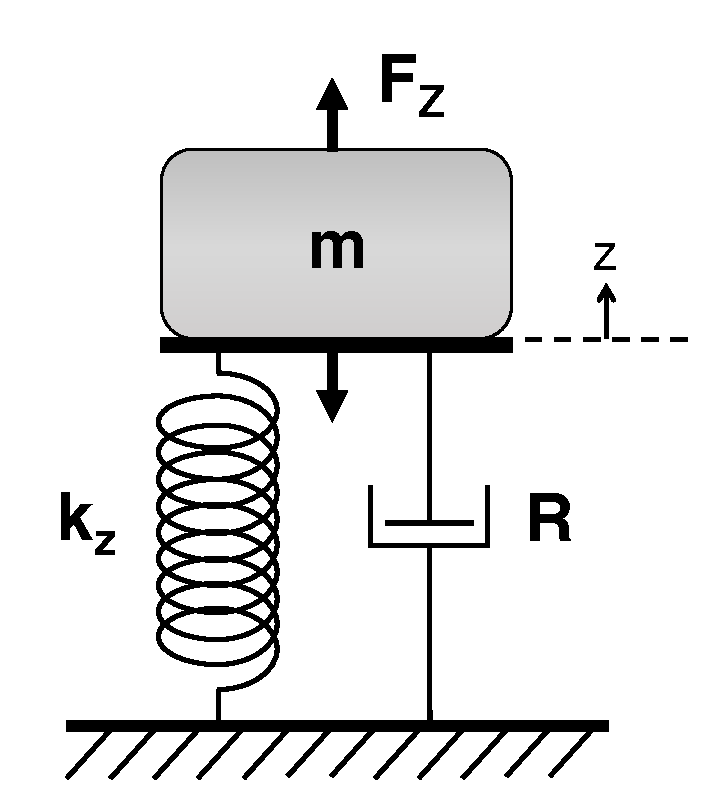
\includegraphics[width=50mm]{SpringSystem.eps}
  \end{minipage}
  \caption{(Left) The experimental setup for the vibration measurements for $D=384$~mm. (Right) Mass-Spring-Damper model.}
  \label{fig:d400}
\end{figure}


\section*{Result and Discussion}

An axial vibration of the rotor can be described by a damping motion of a mass-spring-damper model \cite{mds} shown in the right panel of the Figure \ref{fig:d400}.
The motion of this model is expressed by
\begin{equation}
  m \frac{\partial^{2} x}{\partial^{2} t} + R \frac{\partial x}{\partial t} + k_{z} x = 0,
  \label{eq:damping_motion}
\end{equation}
where $m$ is the mass of the rotor (3.0~kg), $R$ is the damping coefficient and $k_{z}$ is the spring constant.
Under the condition of the damping motion, the solution of the equation (\ref{eq:damping_motion}) is
\begin{equation}
  x = A \mathrm{e}^{- \zeta \omega_{0} t} \cos( \sqrt{1 - \zeta^{2}} \ \omega_{0} t + \phi),
  \label{eq:damping}
\end{equation}
where $\zeta = R / 2 \sqrt{mk_{z}}$ is the damping ratio and $\omega_{0} = \sqrt{k_{z}/m}$ is the undamped angular frequency.
The parameters of $A$ and $\phi$ are the amplitude and the phase determined by the magnitude and the timing of the external impulse force.
Thus, these values are treated as an arbitrary values.

The left panel of the Figure \ref{fig:vibration} shows the laser displacement gauge output and the Hall sensor output as a function of time at the levitation height of 9~mm.
We fit the data with equation (\ref{eq:damping}) and derive the fitting parameters of $\zeta$ and $\omega_{0}$ for each levitation height.
The fitting result of the Hall sensor output with the levitation height of 12~mm is shown the right plot of Figure \ref{fig:vibration}.
The fitted parameters are summarized with their statistical error values in Table \ref{tab:fit_result}.
As a first order, the parameters from the laser displacement gauge and the Hall sensor are consistent.
In an actual application, the measurement by the laser displacement gauge is not ideal from the view points of heat dissipation and interference with the signal.
This result indicates that the Hall sensor can be an alternative to the laser displacement gauge for the vibration measurement.

\renewcommand{\arraystretch}{1.2}
\begin{table}[htbp]
  \centering
  \newcolumntype{Y}{>{\centering\arraybackslash}p{25mm}}
  \begin{tabular}{c|YYYY}
    \hline
    & \multicolumn{4}{c}{laser displacement gauge} \\
    h [mm] & $\zeta$  & $\omega_{0}$ [rad/s] & $R$ [N$\cdot$s/m] & $k_{z}$ [Nm] \\ \hline
    3  & $2.1 \pm 0.3 \times10^{-2}$ & 331.8 $\pm$ 0.8 & 42.0 $\pm$ 5.6 & $3.3 \pm 0.02 \times10^{5}$ \\
    6  & $2.7 \pm 0.1 \times10^{-2}$ & 194.0 $\pm$ 0.2 & 31.0 $\pm$ 2.5 & $1.1 \pm 0.01 \times10^{5}$ \\
    9  & $2.3 \pm 0.1 \times10^{-2}$ & 138.2 $\pm$ 0.2 & 19.1 $\pm$ 2.5 & $5.7 \pm 0.02 \times10^{4}$ \\
    12 & $1.8 \pm 0.1 \times10^{-2}$ & 111.7 $\pm$ 0.1 & 11.8 $\pm$ 1.2 & $3.7 \pm 0.01 \times10^{4}$ \\
    \hline
    & \multicolumn{4}{c}{Hall sensor} \\
    h [mm] & $\zeta$  & $\omega_{0}$ [rad/s] & $R$ [N$\cdot$s/m] & $k_{z}$ [Nm] \\ \hline
    3  & $2.4 \pm 0.1 \times10^{-2}$ & 299.3 $\pm$ 0.2 & 43.5 $\pm$ 2.5 & $2.7 \pm 0.03\times10^{5}$ \\
    6  & $2.3 \pm 0.1 \times10^{-2}$ & 195.7 $\pm$ 0.1 & 27.1 $\pm$ 1.3 & $1.2 \pm 0.01\times10^{5}$ \\
    9  & $2.4 \pm 0.1 \times10^{-2}$ & 136.4 $\pm$ 0.2 & 20.2 $\pm$ 2.8 & $5.6 \pm 0.01\times10^{4}$ \\
    12 & $2.4 \pm 0.1 \times10^{-2}$ & 108.0 $\pm$ 0.1 & 15.7 $\pm$ 0.8 & $3.5 \pm 0.01\times10^{4}$ \\
    \hline
  \end{tabular}
  \caption{The summary of the fitted parameters from the vibration measurements for each levitation height (h). The parameters of $\zeta$ and $\omega_{0}$ represent a damping ratio and an undamped angular frequency. The variables of $R$ and $k_{z}$ represent a damping coefficient and a spring constant.\label{tab:fit_result}}
\end{table}
\renewcommand{\arraystretch}{1.0}

\begin{figure}[htbp]
  \centering
  \begin{minipage}{0.45\hsize}
  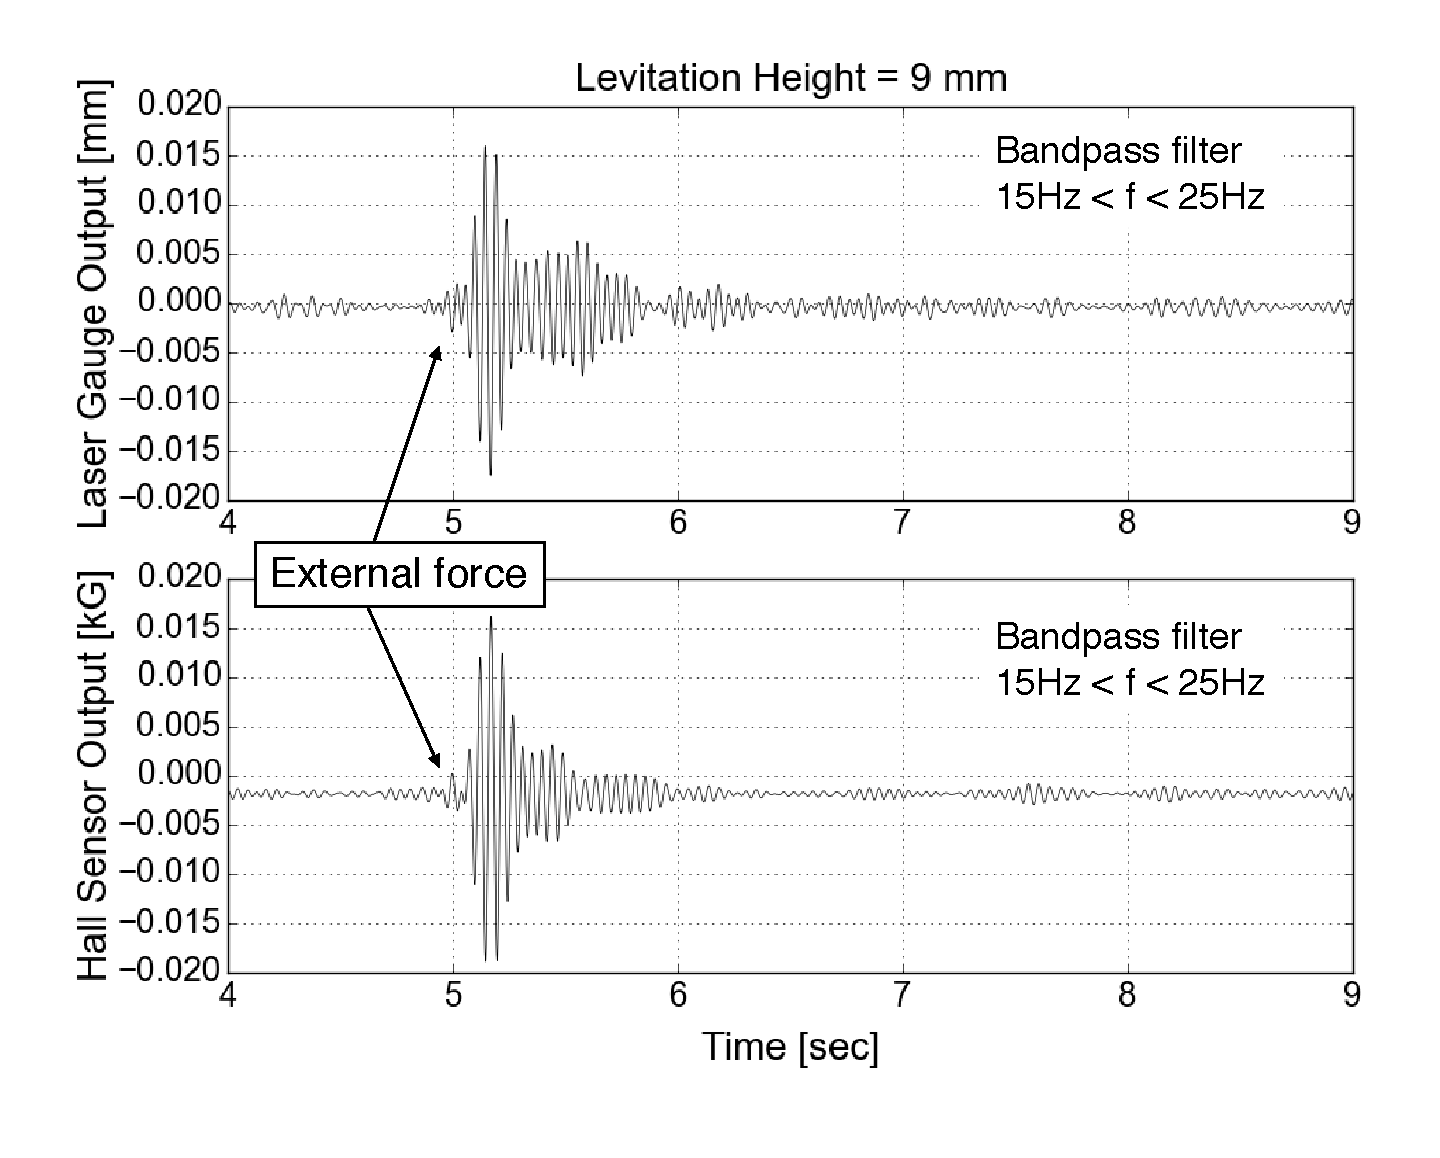
\includegraphics[width=70mm]{vibration_up.eps}
  \end{minipage}
  \begin{minipage}{0.45\hsize}
    \centering
    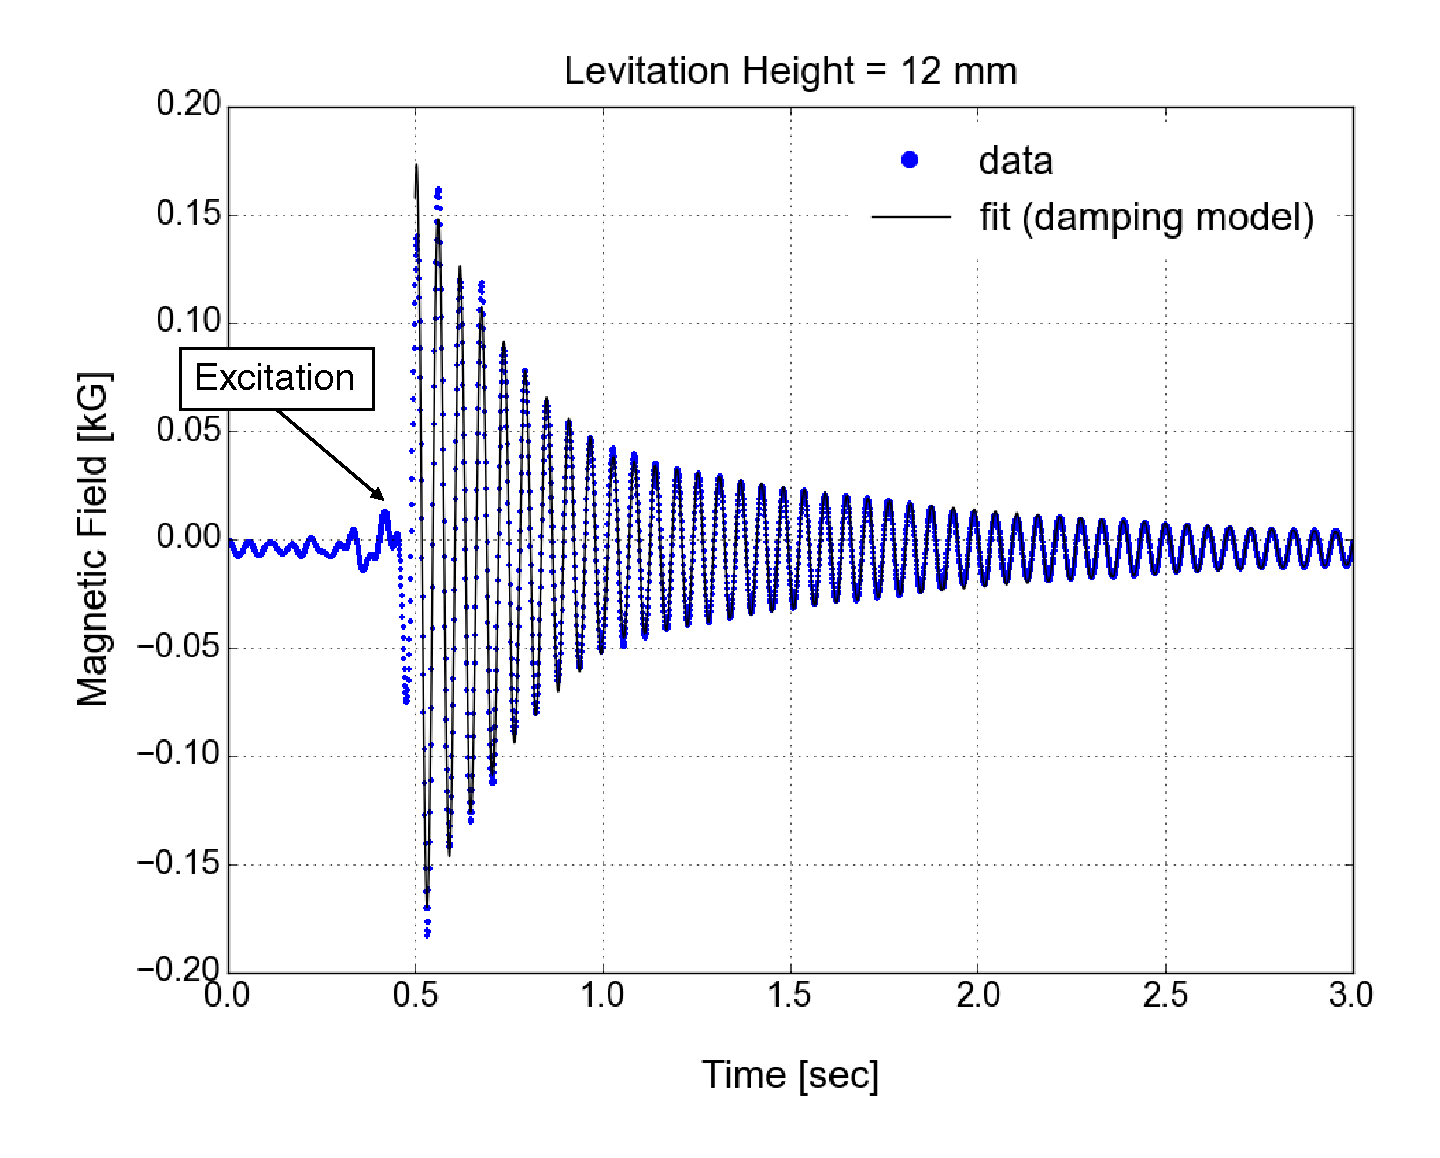
\includegraphics[width=70mm]{vibration_fit.eps}
  \end{minipage}
  \caption{(Left) The laser displacement gauge output and the Hall sensor output as a function of time with the levitation height of 9~mm in top and bottom panels, respectively.
    (Right) The fitting result of the Hall sensor output with the levitation height of 12~mm.}
  \label{fig:vibration}
\end{figure}

We also perform a Fourier transformation to the data from the Hall sensor.
The left panel of the Figure \ref{fig:fft} shows the result of Fourier transformation for each levitation height.
The distinctive peak in the plot corresponds to the natural frequency of the SMB system.
The modulation frequency of the signal by the polarization modulator is less than 20~Hz.
Thus, the natural frequency does not resonate if the levitation height is higher than 12~mm.
The spring constant is also derived calculating by
\begin{equation}
  k_{z} = m (2 \pi f_{0})^{2},
\end{equation}
where $f_{0}$ is the natural frequency of the SMB.
The spring constant from the Fourier transformation is compared with the fitting result in the right panel of the Figure \ref{fig:fft}.
There is no significant difference depending on the analysis method.
For the polarization modulator, the typical requirement of the spring constant is $10^{5}$~Nm.
This SMB system can satisfy the requirement the levitation height is less than 6~mm.

\begin{figure}[htbp]
  \centering
  \begin{minipage}{0.45\hsize}
    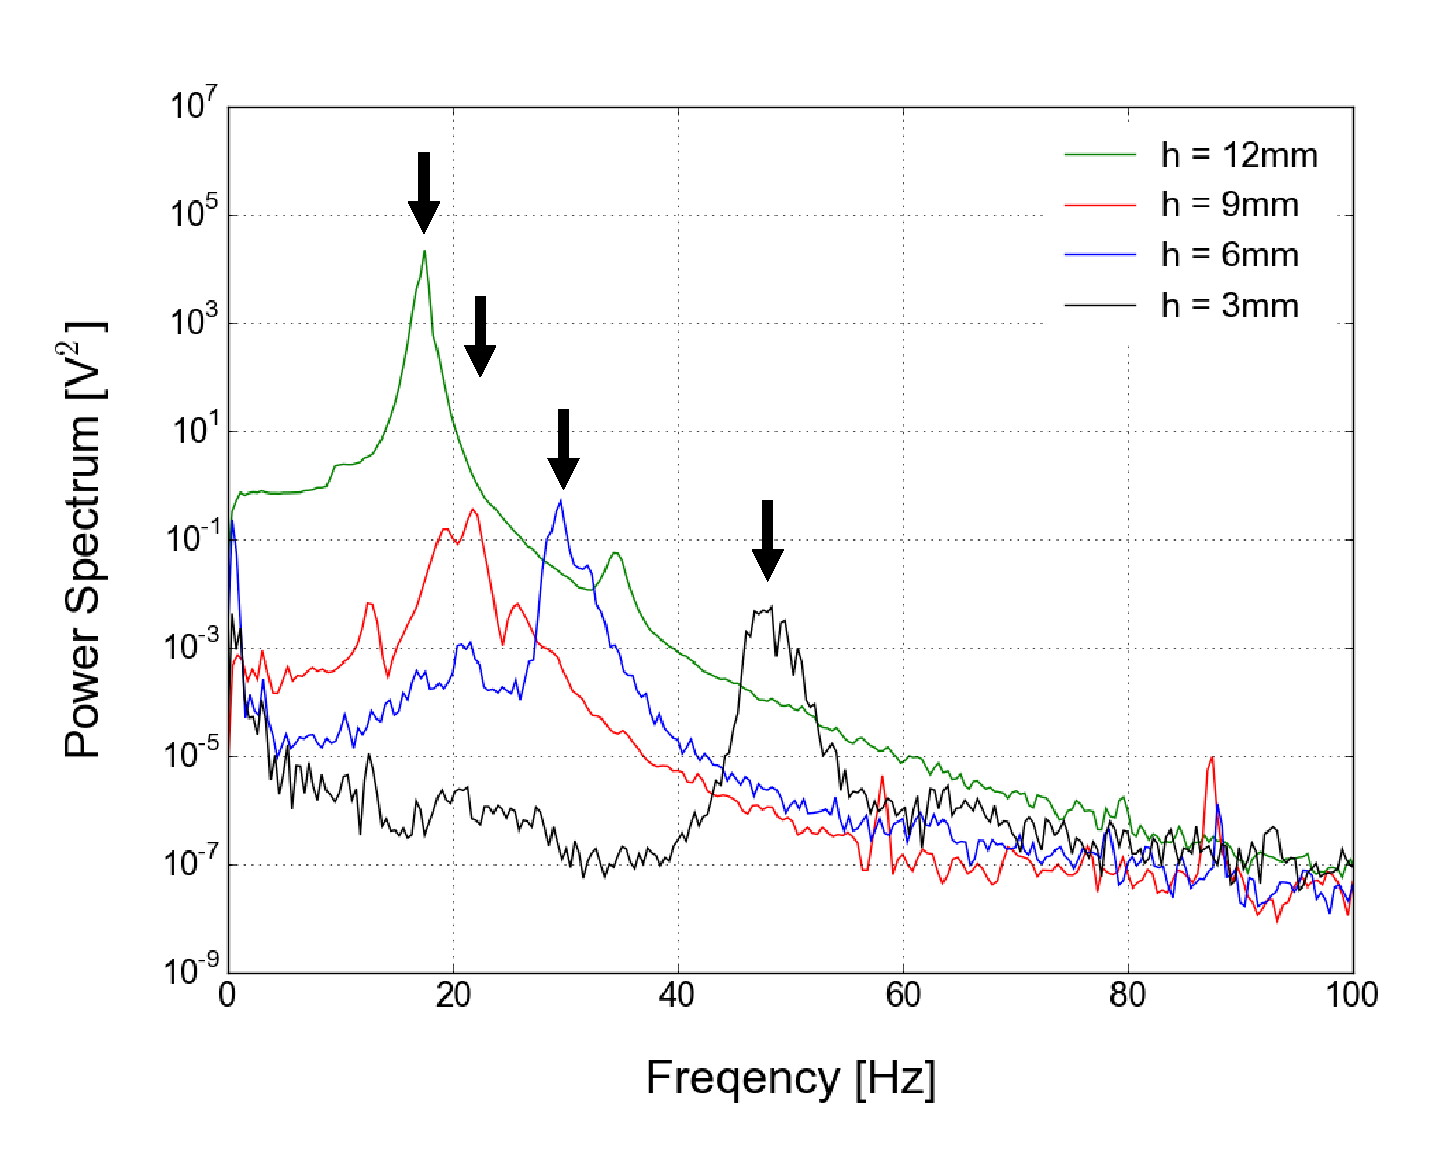
\includegraphics[width=70mm]{vibration_fft_B.eps}
  \end{minipage}
  \begin{minipage}{0.45\hsize}
    \centering
    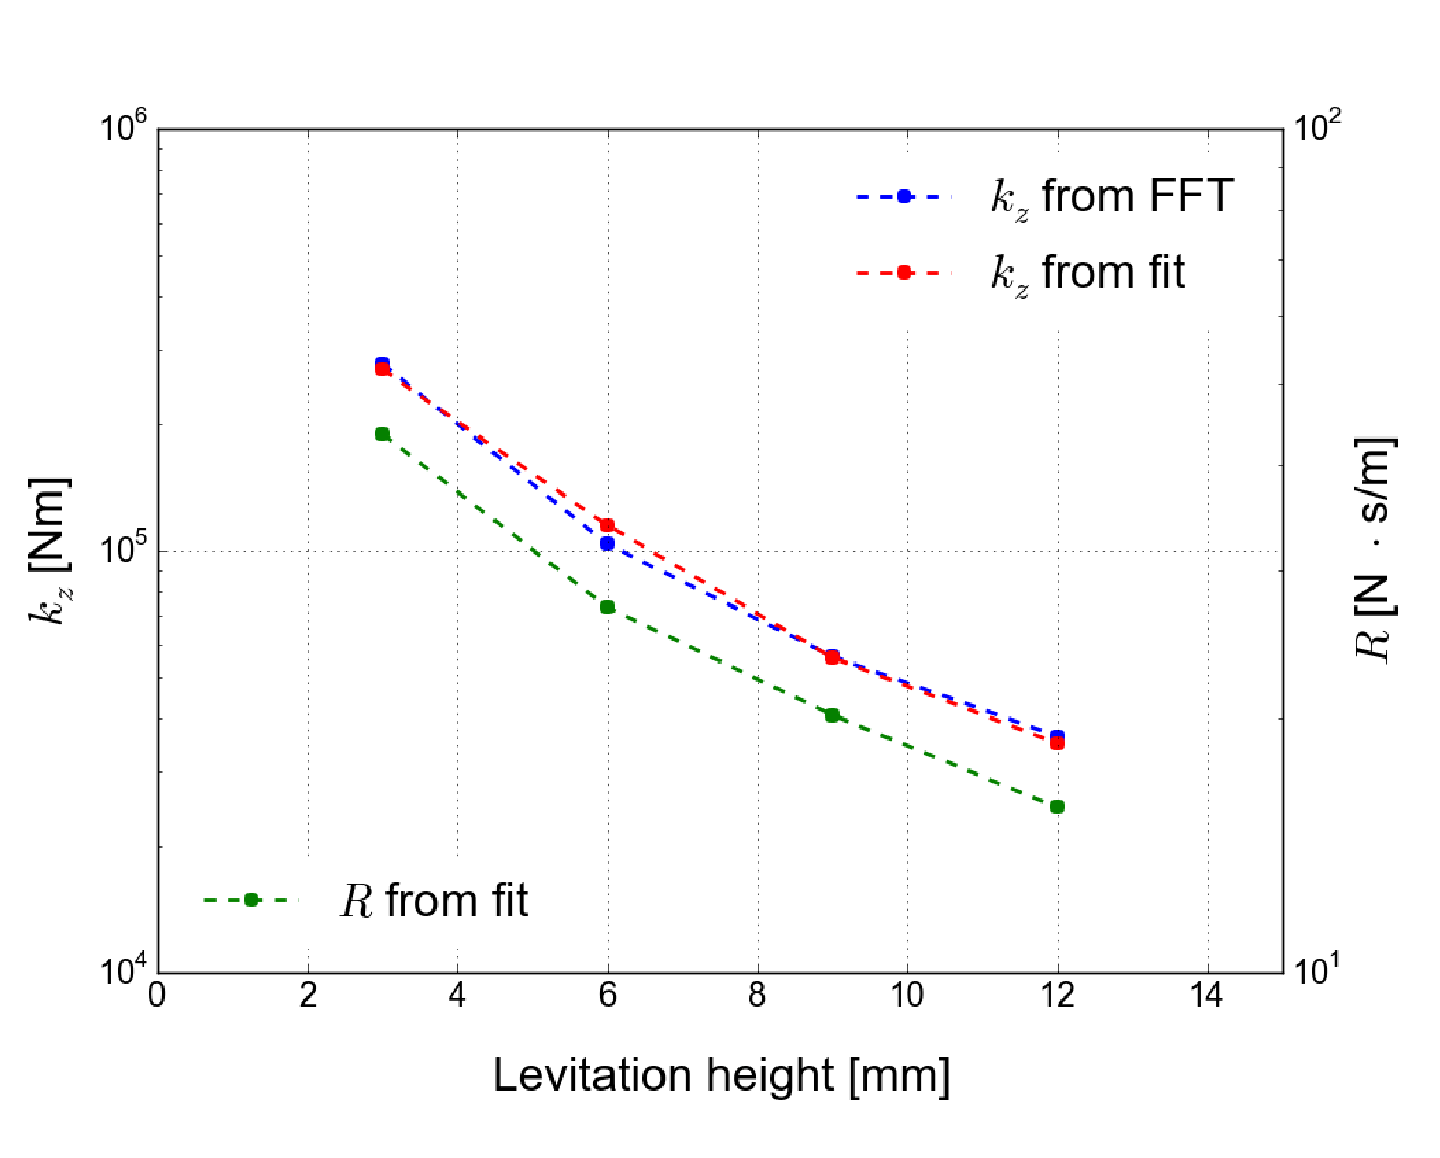
\includegraphics[width=70mm]{SpringConstant.eps}
  \end{minipage}
  \caption{(Left) The power spectrum of the Hall sensor output as a function of frequency for levitation height of 3~mm, 6~mm, 9~mm and 12~mm.
    (Right) The spring constant and the damping coefficient as a function of levitation heights.
    The red and green points are derived from the fit with damping model, and the blue points are derived from the Fourier transformation.}
  \label{fig:fft}
\end{figure}

From this measurement, we demonstrate that the spring constant and the damping coefficient are inversely proportional to the levitation height.
The spring constant corresponds to the stiffness of the SMB.
The damping coefficient corresponds to an energy loss associated with magnetic hysteresis.
From the viewpoint of the stiffness, it is efficient to set the levitation height as less as possible.
However, the increase of the energy loss leads to the noise from the heat dissipation of the HWP.
In addition, The heat dissipation from a magnetic friction during the rotation also increases by reducing the levitation height.
Thus, the SMB system has a trade-off between the stiffness and the heat dissipation.
For the polarization modulator, the levitation height of the SMB is an important parameter to be determine by the experimental requirement.
In this measurement, we use the segmented ring magnet with axial magnetization.
The further effort of designing an optimal magnetic circuit can be improve the total performance of the SMB system.
The measurement and evaluation of the magnetic circuit will be discussed in future papers.

\section*{Conclusion}
We have conducted the vibration measurements of the prototype SMB system with the diameter of $\phi$=384~mm for the polarization modulator used in CMB polarization experiments.
From the measurement, we derive the spring constant and the damping coefficient using both the laser displacement gauge and the cryogenic Hall sensor.
The spring constant is in the order of $10^{4} \sim 10^{5}$~Nm and the damping coefficient is $15\sim45$ depending on levitation height.
The result has consistency between the laser gauge and the Hall sensor.
We conclude that the Hall sensor can be an alternative method to monitor the vibration of the SMB system.
We also discuss the trade-off of the SMB system between the stiffness and the heat dissipation.
We demonstrate the stiffness and the heat dissipation is possible to control by the levitation height.
The further effort of designing an optimal magnetic circuit can be improve the total performance of the SMB system.

\section*{Acknowledgment}
The author would like to thank to Dr. H. Imada at ISAS/JAXA.
This work was supported by MEXT KAKENHI Grant Numbers JP15H05441 and JSPS Core-to-Core Program, A. Advanced Research Networks.
This work was also supported by World Premier International Research Center Initiative (WPI), MEXT, Japan.


\vspace*{5mm}
\begin{thebibliography}{99}

\bibitem{inflation_sato}
Sato K, First-order phase transition of a vacuum and the expansion of the Universe, {\it Monthly Notices of Royal Astronomical Society}, {\bf 195}, 467, (1981).
\bibitem{inflation_guth}
Guth Alan H, The Inflationary Universe: A Possible Solution to the Horizon and Flatness Problems, {\it Phys. Rev. D} {\bf 23}, 347 (1981).
\bibitem{smb}
Hull J, TOPICAL REVIEW: Superconducting bearings, {\it  Superconductor Science and Technology}, {\bf 13}, Issue 2, pp. R1-R15 (2000).
\bibitem{ebex}
Klein J et al., A cryogenic half-wave plate polarimeter using a superconducting magnetic bearing, {\it Proceedings of the SPIE, Cryogenic Optical Systems and Instruments XIII}, Volume 8150, 815004 (2011).
\bibitem{litebird}
Masumura T et al., LiteBIRD: mission overview and design tradeoffs, {\it Proceedings of the SPIE, Space Telescopes and Instrumentation 2014}, Volume 9143, 91431F (2014).
\bibitem{matsumura_eucas2015}
Matsumura T, Kataza H, Utsunomiya S, Yamamoto R, Hazumi M, Katayama N, Design and Performance of a Prototype Polarization Modulator Rotational System for Use in Space Using a Superconducting Magnetic Bearing, { \it IEEE Transactions on Applied Superconductivity}, Volume: 26, Issue 3, (2016).
\bibitem{Hull}
Hull J, Cansiz A, Vertical and lateral forces between a permanent magnet and a high-temperature superconductor, {\it Journal of Applied Physics}, Volume 86, Issue 11 (1999).
\bibitem{mds}
Takahata R, Ueyama H, Characterization of Superconducting Magnetic Bearings (Vibration Damping and Hysteresis of Magnetic Force in Superconductor), {\it Advances in Superconductivity IV}, pp 1089-1092 (1992).

\end{thebibliography}


\end{document}



% LocalWords:  Sakurai Tomotake Sugai Katayama
